%\section{Conceptos necesarios}
En esta sección se introducen brevemente los conceptos que son necesarios para comprender el trabajo realizado.
\section{Metodologías ágiles}

Las metodologías ágiles describen un enfoque general para el desarrollo de productos y la gestión de proyectos. Tienen un enfoque flexible que está centrado en el cliente y su colaboración con equipos de desarrollo. Los equipos que utilizan estas metodologías construyen y entregan pequeñas partes de funcionalidad del producto de forma incremental e iterativa. Luego, los equipos ajustan lo que entregarán a continuación basándose en la retroalimentación de los clientes y de los principales interesados.
\cite{cohan_agile}
\section{Historias de usuario}
Una historia de usuario es un escenario: una descripción de un uso (potencial) real de un sistema. Se plantea desde la perspectiva del cliente o del usuario y representa el entendimiento compartido de un equipo sobre lo que el sistema debería hacer.\cite{wake_definition}

Una de las plantillas utilizadas para la redacción de historias de usuario es: Como un tipo de usuario, quiero hacer algo para que se cumpla algún objetivo. Está compuesta entonces por un Rol, una Acción y Contexto o Propósito
\subsection{Criterios de aceptación}

Los criterios de aceptación complementan las historias de usuario agregando detalles como condiciones específicas que deben cumplirse para que una historia sea aceptada como completa. \cite{cohan_details}

Por ejemplo dada la historia: Como usuario, puedo iniciar sesión a través de una cuenta de redes sociales.

Posibles criterios de aceptación serian:
\begin{itemize}
    \item Puede iniciar sesión a través de Facebook
    \item Puede iniciar sesión a través de LinkedIn
    \item Puede iniciar sesión a través de Twitter
\end{itemize}

\subsection{Épicas}
Una épica es una historia de usuario grande que normalmente no puede completarse en una sola iteración y que debe dividirse en varias historias de usuario más pequeñas.\cite{cohan_epic}

Por ejemplo la historia: Como usuario autorizado, puedo ejecutar reportes para poder ver el estado financiero de la organización.

Puede dividirse en diferentes tipos de reportes financieros:
\begin{itemize}
  \item Como usuario autorizado, puedo ejecutar un reporte de pérdidas y ganancias.
  \item Como usuario autorizado, puedo ejecutar un reporte de flujo de caja.
  \item Como usuario autorizado, puedo ejecutar un reporte detallado de transacciones.
\end{itemize}

\section{Inteligencia Artificial}
La inteligencia artificial (IA) abarca una gran variedad de campos, que van desde los más generales (como el aprendizaje y la percepción) hasta otros más específicos, como jugar ajedrez, demostrar teoremas matemáticos, escribir poesía, conducir un automóvil en una calle concurrida y diagnosticar enfermedades. \cite{IABook} En la Tabla \ref{table:defIA} se presentan ocho definiciones de inteligencia artificial.

\begin{table}[h!]
\label{table:defIA}
\centering
\begin{tabular}{|p{6cm}|p{6cm}|}
\hline
\textbf{Pensar como humanos} & \textbf{Pensar racionalmente} \\ \hline

“El emocionante nuevo esfuerzo por hacer que las computadoras piensen... máquinas con mente, en el sentido pleno y literal.” (Haugeland, 1985)

“La automatización de actividades que asociamos con el pensamiento humano, actividades como la toma de decisiones, la resolución de problemas y el aprendizaje.” (Bellman, 1978)

&
“El estudio de las facultades mentales mediante el uso de modelos computacionales.” (Charniak y McDermott, 1985)

“El estudio de los cálculos que hacen posible percibir, razonar y actuar.” (Winston, 1992)
\\ \hline

\textbf{Actuar como humanos} & \textbf{Actuar racionalmente} \\ \hline

“El arte de crear máquinas que realizan funciones que requieren inteligencia cuando son realizadas por personas.” (Kurzweil, 1990)

“El estudio de cómo hacer que las computadoras hagan cosas en las que, por el momento, las personas son mejores.” (Rich y Knight, 1991)

&
“La inteligencia computacional es el estudio del diseño de agentes inteligentes.” (Poole et al., 1998)

“La IA se ocupa del comportamiento inteligente en artefactos.” (Nilsson, 1998)
\\ \hline

\end{tabular}
\caption{Figura 1.1 de Artificial Intelligence: A Modern Approach: Algunas definiciones de inteligencia artificial organizadas en cuatro categorías. }
\end{table}

\subsection{Modelos}
En la actualidad, la IA está experimentando un cambio de paradigma con el surgimiento de modelos (por ejemplo, BERT, DALL-E, GPT-3) entrenados con datos amplios (generalmente utilizando autoaprendizaje a gran escala) que pueden adaptarse a una amplia gama de tareas posteriores. \cite{bommasani2021foundation}. La Figura \ref{fig:model} ilustra esto.
\newpage
\begin{figure}[h!]
    \centering
    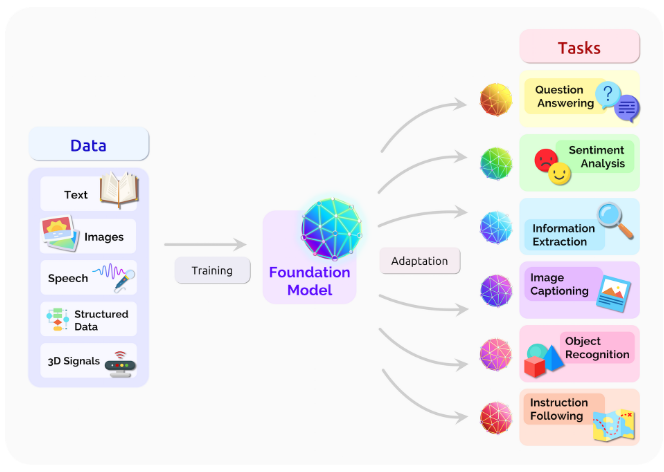
\includegraphics[width=\textwidth]{figs/model.png}
    \caption{Figura 2 de On the Opportunities and Risks of
Foundation Models: Un modelo base puede centralizar la información de todos los datos provenientes de diversas modalidades. Este único modelo luego puede adaptarse a una amplia gama de tareas posteriores.}
    \label{fig:model}
\end{figure}


\subsection{Grandes modelos de lenguaje}
El procesamiento de lenguaje natural (NLP) es el campo de la inteligencia artificial que se ocupa de permitir que las computadoras comprendan y procesen lenguajes humanos. \cite{IABook}

Los modelos de lenguaje son aquellos aplicados al campo del procesamiento del lenguaje natural. Actualmente, los grandes modelos de lenguaje o Large Language Models (LLM) son los más utilizados. Son utilizados en tareas de generación de texto, como la elaboración de resúmenes y la generación de diálogos \cite{bommasani2021foundation}.

En 2020 el articulo Language Models are Few-Shot Learners \cite{brown2020language} presento el modelo GPT-3, que popularizo el uso de la Inteligencia Artificial en los años siguientes.\cite{miller2023artificial}

\subsection{Instrucción (Prompt)}

Para utilizar los modelos en tareas de predicción, la entrada original x se modifica mediante una plantilla para convertirla en una cadena de texto prompt x' que contiene algunos espacios sin completar y luego se utiliza el modelo de lenguaje para llenar probabilísticamente la información faltante. \cite{liu2021prompting}

En términos simples, un prompt es un texto en lenguaje natural que indica de alguna manera la tarea que la inteligencia artificial debe realizar. 

Por ejemplo en la figura \ref{fig:ejemplo_prompt} se ejemplifica un prompt Traducir al ingles, que indica la traducción en ingles de la frase Hola Mundo.

\begin{figure}[h!]
    \centering
    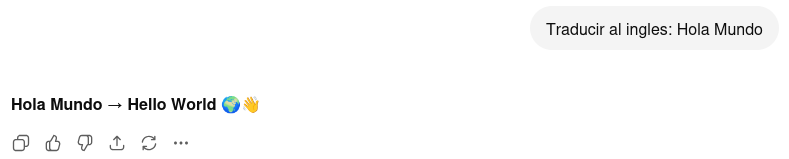
\includegraphics[width=\textwidth]{figs/ejemploprompt.png}
    \caption{Ejemplo de prompt para la traducción en Ingles}
    \label{fig:ejemplo_prompt}
\end{figure}
